\documentclass{article}
\usepackage{amsmath}
\usepackage{geometry}
\usepackage{tikz}
\usetikzlibrary{shapes,arrows,positioning}
\usepackage{booktabs}
\usepackage{graphicx}
\usepackage{subcaption}
\usepackage{multirow}

\begin{document}

\title{A Novel Surrogate Modeling Framework for Activated Sludge Processes using Coupled Bilinear Regression Equations}

\maketitle

\section{Introduction}

Water pollution presents a critical environmental and public health challenge worldwide, with particularly severe repercussions in developing nations (Lin et al., 2022; Madhav et al., 2020). Biological wastewater treatment systems, particularly those based on the activated sludge process, are the dominant approach applied to combat this issue (Duan et al., 2022). However, their modeling and analysis present formidable engineering and computational challenges (Xiao et al., 2025). The underlying biophysical mechanisms are governed by the Activated Sludge Models (ASM) (Henze et al., 2006), which rely on coupled, multiplicative non-linear kinetic expressions (e.g., Monod functions) to describe microbial growth and substrate consumption. This inherent non-linearity limits the practical application of transparent analytical methods for process design and control of these systems, frequently forcing engineers to rely on iterative trial-and-error approaches or computationally expensive heuristic algorithms (Aboagye et al., 2021; Padron-Paez et al., 2020).

In response to this complexity, research has increasingly focused on developing surrogate models to approximate the behavior of these systems (Bhosekar \& Ierapetritou, 2018; Durkin et al., 2024). Traditional approaches have explored linearization techniques, such as Taylor series expansion (M. Li et al., 2020; T. Yang et al., 2014). While computationally efficient for optimal control applications, these methods severely restrict the search space required for comprehensive process design analysis because the model is only valid around the vicinity of the approximation point. Another category involves multivariable polynomial fitting (Ahn et al., 2014; Kim et al., 2009; Lim et al., 2011). However, these simpler models often fail to capture the complex interdependencies among wastewater constituents, ignoring the stoichiometric constraints inherent in biological reactions. On the other hand, multivariate statistical approaches such as Partial Least Squares Regression (PLS) are widely used in this domain as a robust alternative to simple regression (Khatri et al., 2020). PLS is particularly suited for water quality analysis, i.e., effluent prediction, because it effectively handles the high dimensionality and multicollinearity inherent in wastewater datasets (Wold et al., 2001). By projecting the input and output matrices to a lower-dimensional space of latent variables, PLS can extract useful information from correlated predictors, such as the relationships between BOD, COD, and various nitrogen species (Khatri et al., 2020). However, it has not yet been applied to simultaneously capture the highly coupled and synergistic nature of the biological state and hydrodynamic variables in wastewater treatment systems.

On the other hand, the machine learning (ML) paradigm has emerged as a promising alternative, capable of mapping highly non-linear relationships (Croll et al., 2023; Nazlabadi et al., 2021). Several studies have deployed ML techniques to model activated sludge processes (Sin \& Al, 2021). For instance, Support Vector Machines (SVM) trained on simulation data have been used to predict effluent quality (Fang et al., 2011). Similarly, Artificial Neural Networks (ANN), Random Forests, and k-Nearest Neighbors (k-NN) have been investigated for modeling specific aspects of the aeration process (Asadi et al., 2017; Henao \& Maravelias, 2011; Mao et al., 2024). Several other ML models like XGBoost (Yang et al., 2025), LightGBM (Wang et al., 2025), and Support Vector Regression (SVR) (Moghaddam \& Mesghali, 2023) have been applied for predicting effluent concentration in wastewater treatment. However, while these non-linear ML models offer high fidelity, they frequently act as "black boxes." They obscure the mathematical relationship between inputs and outputs, making it difficult to discern which interactions drive the predictions. Furthermore, their high parameter density can lead to overfitting, where the model captures noise rather than the underlying signal, limiting their interpretability for engineering analysis.

These limitations underscore a critical gap: the lack of a modeling framework that combines the high predictive accuracy of advanced ML algorithms with an algebraic structure that balances complexity with interpretability. This study introduces the Coupled Bilinear Regression Equations (CoBRE) as a new surrogate modeling framework designed to address this need. The mathematical underpinnings of the CoBRE are not entirely new. Bilinear models have a long history in control theory and econometrics (Kim et al., 2022). However, the novelty of this work lies in the specific adaptation and application of this algebraic structure to the domain of biological wastewater treatment. Unlike other bilinear systems, the CoBRE presented here is structurally modified to explicitly account for the stoichiometric coupling and hydrodynamic gain modulation, which are essential in modeling biological wastewater treatment systems. Thus, we leverage the known algebraic properties of bilinear regression equations while tailoring it to approximate the specific non-linearities of the ASM. This yields a parsimonious, high-fidelity surrogate that remains algebraically interpretable, offering a middle ground between rigid mechanistic models and opaque machine learning algorithms.

The primary objective of this article is to rigorously compare the predictive performance of the CoBRE against a comprehensive suite of established algorithms utilized in wastewater modeling. This suite includes PLS as a robust statistical baseline, distance-based algorithms (k-NN), kernel-based methods (SVR), and advanced ensemble and deep learning techniques (Random Forest, XGBoost, LightGBM, and ANN). The focus of this comparative analysis is the Activated Sludge Process, examining both a standalone Continuous Stirred Tank Reactor (CSTR) unit and a full activated sludge plant configuration. By demonstrating competitive predictive performance and computational tractability, this research aims to establish the CoBRE as a viable surrogate candidate, providing the necessary empirical foundation for future work focused on process analysis.

\section{Theory and Calculation}
\subsection{Nomenclature}
The variables and coefficients used in the formulation of the CoBRE are defined as follows.

\begin{itemize}
    \item $k, p$: Indices representing the dependent composite state variables (e.g., COD, TN, TSS).
    \item $m, i, j$: Indices representing the independent input variables. Note: For a specific unit operation, $x_{m}$ includes both operational set-points and the influent composite concentrations entering that specific unit.
    \item $y_{k}$: The scaled, log-transformed value of the dependent composite variable $k$.
    \item $x_{m}$: The scaled value of the independent input variable $m$.
    \item $\Upsilon_{k}$: The regression intercept for variable $k$, representing the baseline system response.
    \item $B_{km}$: The linear coefficient matrix quantifying the direct proportional effect of input $m$ on output $k$.
    \item $\Theta_{k,ij}$: The tensor coefficient quantifying the synergistic or inhibitory interaction between two independent inputs $x_{i}$ and $x_{j}$ on output $k$.
    \item $\Gamma_{kp}$: The coupling coefficient matrix quantifying the statistical dependency of composite $k$ on another composite $p$.
    \item $\Lambda_{km}$: The bilinear coefficient matrix quantifying the gain-scheduling effect of input $m$ on the response of $k$.
    \item $C_{k}$: The actual physical concentration of component $k$ (mg/L).
    \item $\mu_{k}, \sigma_{k}$: The mean and standard deviation used to normalize the log-transformed physical concentrations.
\end{itemize}

\subsection{Model Derivation}
The CoBRE is constructed by systematically introducing algebraic terms that mimic the fundamental physical and biochemical phenomena observed in wastewater treatment units. The model predicts the state $y_{k}$ implicitly.

The foundation of the model is a linear approximation. In many transport phenomena, an increase in mass loading (input) leads to a proportional increase in effluent concentration (output). This linear relationship is captured by the intercept and the term $B_{km}$:

\begin{equation}
\text{Linear Effect: } \quad \Upsilon_{k} + \sum_{m} B_{km} x_{m}
\end{equation}

However, biological systems exhibit complex non-linearities that a simple linear model cannot capture. The first critical non-linearity is the interaction between operational inputs. For example, the rate of nitrification (reduction in TKN) depends simultaneously on the concentration of nitrogen and the availability of dissolved oxygen. If either is zero, the reaction stops. To capture this synergistic behavior, the CoBRE introduces the term $\Theta_{k,ij}$, which accounts for the product of two inputs:

\begin{equation}
\text{Input Synergies: } \quad \sum_{i} \sum_{j} \Theta_{k,ij} (x_{i} x_{j})
\end{equation}

A positive $\Theta_{k,ij}$ indicates that the combined presence of inputs $x_{i}$ and $x_{j}$ enhances the process beyond the sum of their individual effects, effectively mimicking the multiplicative nature of Monod kinetic terms (Henze et al., 2006).

The second critical feature is the coupling between composite variables. In the ASM, the consumption of substrate (COD) is strictly tied to the removal of nutrients (TN, TP) via stoichiometry (Barker \& Dold, 1997; Henze et al., 1999). In the CoBRE, this is modeled via the coupling term $\Gamma_{kp}$, which links the dependent variable $y_{k}$ to other state variables $y_{p}$:

\begin{equation}
\text{Stoichiometric Coupling: } \quad \sum_{p} \Gamma_{kp} y_{p}
\end{equation}

It is important to clarify the physical interpretation of this term in the context of composite variables. Unlike the strict mass balances of the ASM species, the $\Gamma_{kp}$ term here captures the statistical correlations driven by underlying biological mechanisms. For instance, a high removal of TN (denitrification) is physically coupled with the consumption of COD. Therefore, the model can "learn" that low effluent TN is correlated with lower effluent COD, provided sufficient carbon was available. Furthermore, it should be emphasized that the CoBRE framework is not mathematically restricted to modeling composite variables. In principle, the model can be formulated using the granular state variables of the ASM (e.g., $S_{S}$, $X_{S}$, $X_{BH}$) without loss of generality. The decision to constrain the current discussion to composite indicators is driven by the practical necessity of aligning with sensor capabilities and regulatory standards, which has been a mainstream approach to surrogate modeling carried out in the literature (Xiao et al., 2025; Durkin, Otte, \& Guo, 2024; Bhosekar \& Ierapetritou, 2018; Henao \& Maravelias, 2011; Caballero \& Grossmann, 2008). 

The final and most distinct term addresses the hydrodynamic non-linearity of the system. In CSTRs, the system gain—how strongly the output responds to a change in reaction rate—is modulated by the hydraulic retention time. As the influent flow rate increases, the retention time decreases, potentially leading to "washout" where biomass cannot be sustained. This implies that the state variable $y_{k}$ itself depends on the input flow rate $x_{m}$. This is modeled by the bilinear term $\Lambda_{km}$:

\begin{equation}
\text{Gain Modulation: } \quad \sum_{m} \Lambda_{km} (y_{k} x_{m})
\end{equation}

By combining these terms, we arrive at the full formulation of the CoBRE. The conceptual framework of these interactions is illustrated in Figure~\ref{fig:cobre-conceptual}. The equation is arranged implicitly, grouping the dependent variable $y_{k}$ and its coupled terms on the left-hand side, and the independent forcing functions on the right-hand side:

\begin{equation}
y_{k} - \sum_{m} \Lambda_{km} (y_{k} x_{m}) - \sum_{p} \Gamma_{kp} y_{p} = \Upsilon_{k} + \sum_{m} B_{km} x_{m} + \sum_{i} \sum_{j} \Theta_{k,ij} (x_{i} x_{j})
\end{equation}

\begin{figure}[h]
\centering
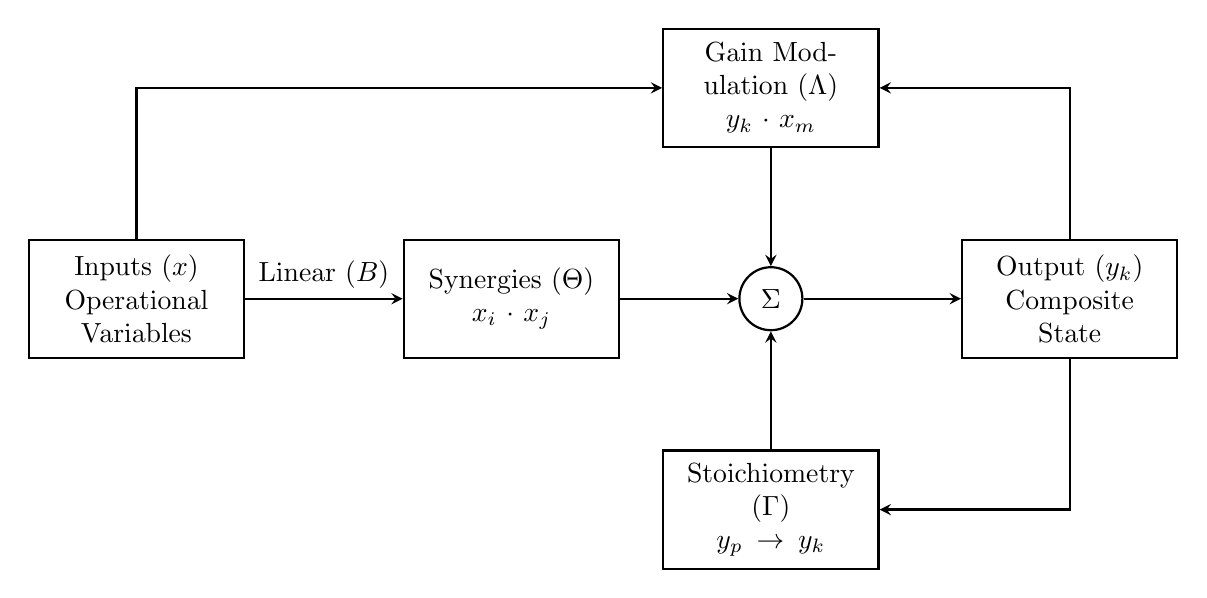
\begin{tikzpicture}[node distance=2cm, auto, >=stealth, thick]
    % Styles
    \tikzstyle{block} = [rectangle, draw, fill=white, text width=2.5cm, text centered, minimum height=1.5cm]
    \tikzstyle{sum} = [circle, draw, fill=white, node distance=1cm, minimum size=0.8cm]
    \tikzstyle{line} = [draw, ->]

    % Nodes
    \node [block] (input) {Inputs ($x$) \\ Operational Variables};
    \node [block, right=2cm of input] (interactions) {Synergies ($\Theta$) \\ $x_{i} \cdot x_{j}$};
    \node [sum, right=1.5cm of interactions] (summation) {$\Sigma$};
    \node [block, below=1.5cm of summation] (coupling) {Stoichiometry ($\Gamma$) \\ $y_{p} \to y_{k}$};
    \node [block, above=1.5cm of summation] (gain) {Gain Modulation ($\Lambda$) \\ $y_{k} \cdot x_{m}$};
    \node [block, right=2cm of summation] (output) {Output ($y_{k}$) \\ Composite State};

    % Edges
    \path [line] (input) -- node[above] {Linear ($B$)} (interactions);
    \path [line] (interactions) -- (summation);
    \path [line] (summation) -- (output);
    \path [line] (coupling) -- (summation);
\path [line] (gain) -- (summation);
    
    % Feedback loops indicating coupling
    \draw [->] (output.south) |- (coupling.east);
    \draw [->] (output.north) |- (gain.east);
\draw [->] (input.north) |- (gain.west);

\end{tikzpicture}
\caption{Conceptual framework of the Coupled Bilinear Regression Equations (CoBRE). The model predicts the output state $y_{k}$ by aggregating linear inputs, non-linear input synergies, stoichiometric coupling from other states, and hydrodynamic gain modulation. Note that the feedback loops indicated represent algebraic coupling between variables in the steady-state solution, not time-delay dynamic feedback.}
\label{fig:cobre-conceptual}
\end{figure}

It is pertinent to discuss why we opted to model the CoBRE specifically as a bilinear system. In principle, the approximation could be generalized to maximize the number of variables coupled together, creating a high-dimensional polynomial representation just like that of the TaylorFit model, which, just like the CoBRE, is also based on multivariate polynomial regression (Jagupilla et al., 2020). Such a generalized mathematical structure, which accounts for interactions of arbitrary order $D$, can be expressed using the following operator notation:

\begin{equation}
y_{k} = \Upsilon_{k} + \sum_{p} \Gamma_{kp} y_{p} + \sum_{d=2}^{D} \sum_{i_{1}} \cdot \cdot \cdot \sum_{i_{d}} \Theta^{(d)}_{k, i_{1} \cdot \cdot \cdot i_{d}} ( \prod_{j=1}^{d} x_{i_{j}} ) + \sum_{d=1}^{D} \sum_{p} \sum_{i_{1}} \cdot \cdot \cdot \sum_{i_{d}} \Lambda^{(d)}_{kp, i_{1} \cdot \cdot \cdot i_{d}} ( y_{p} \prod_{j=1}^{d} x_{i_{j}} )
\end{equation}

In this generalized form, the term $\Theta^{(d)}$ represents a high-order tensor capturing pure input interactions (e.g., $x_{1} x_{2} x_{3}$ for $d=3$), while $\Lambda^{(d)}$ captures high-order gain modulation where the state $y_{p}$ is influenced by a product of multiple inputs (e.g., $y_{p} x_{1} x_{2}$). While this higher-order structure theoretically increases the flexibility of the model, the bilinear structure adopted in Equation 5 is deliberate. We restrict the model to pairwise interactions ($x_{i} x_{j}$ and $y_{k} x_{m}$) to ensure parsimony, which is critical for two reasons. First, restricting the expansion to bilinear terms significantly reduces the potential for overfitting. As the order $d$ increases, the number of coefficients in tensors $\Theta^{(d)}$ and $\Lambda^{(d)}$ explodes combinatorially, often capturing noise rather than physical signal. Second, and most critically, minimizing the degree of non-linearity directly impacts the interpretability and statistical robustness of the model.

The restriction to bilinear terms is a deliberate modeling choice to balance flexibility with parsimony. While the CoBRE is a statistical approximation and does not strictly enforce the mechanisms of the ASM, its algebraic structure is designed to emulate the phenomenological behavior of biological systems. Kinetic rates in wastewater treatment are often driven by multiplicative factors (e.g., biomass concentration $\times$ substrate concentration). By limiting the expansion to bilinear terms, the model captures the statistical signature of these dominant interactions without the combinatorial explosion of coefficients associated with higher-order polynomial fitting. This reduces the risk of overfitting and ensures the model remains a compact, interpretable approximation of the complex underlying process.

\section{Methodology}

The development of the CoBRE and its comparative analysis against established ML paradigms relies on a rigorous computational framework. As the acquisition of extensive, noise-free datasets spanning the entire design space of biological wastewater treatment is practically infeasible in physical facilities, this study employs high-fidelity biophysical process simulation. This approach aligns with recent trends in the literature where simulation packages like GPS-X, Biowin, and AQUASIM are used to generate comprehensive datasets for ML training (Bazemo et al., 2021; Bressani-Ribeiro et al., 2021; Caro et al., 2024; Durkin et al., 2024). Specifically, Durkin et al. (2024) demonstrated the efficacy of harnessing high-fidelity data from black-box process simulations to train surrogate models for superstructure analysis, validating the approach of using simulation data to overcome the computational intractability of rigorous models.

\subsection{Biophysical Process Simulation}
The training and validation datasets were generated using the QSDsan framework (Li et al., 2022). QSDsan is a popular Python-based modeling framework that has been utilized for various wastewater treatment research and applications (Zhang et al., 2025; Lohman et al., 2023). The biophysical system was modeled using the Activated Sludge Model No. 2d (ASM2d) (Henze et al., 1999) to capture carbon oxidation, nitrification, denitrification, and biological phosphorus removal.

To create a diverse and generalized dataset, we constructed a process flowsheet consisting of five CSTRs arranged in series, followed by a secondary clarifier. A critical innovation in this data generation strategy is the decoupling of these units from fixed operational definitions. The metabolic state of each reactor was not pre-assigned but rather determined dynamically by the input conditions. Specifically, the oxygen mass transfer coefficient ($K_{L}a$) for every reactor was treated as a stochastic variable. By allowing $K_{L}a$ to vary randomly between 0 and 800 d$^{-1}$ for all units, the simulation captures a continuous spectrum of oxygenation conditions across the treatment train. A schematic of the generalized superstructure is provided in Figure~\ref{fig:superstructure}.

\begin{figure}[h]
\centering
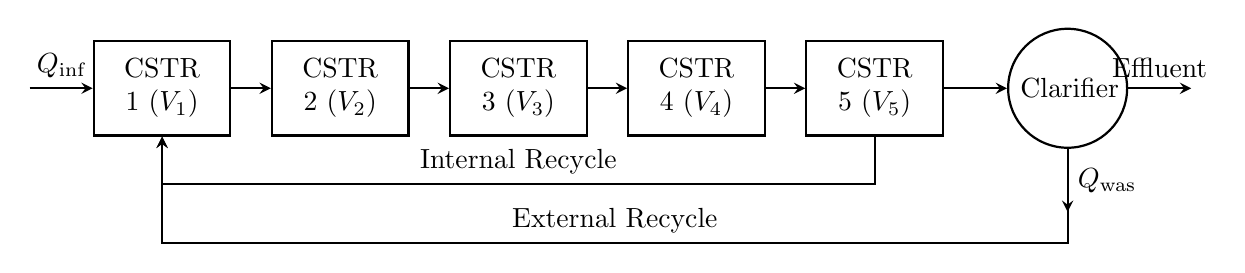
\begin{tikzpicture}[node distance=1.5cm, auto, >=stealth, thick]
    % Styles
    \tikzstyle{block} = [rectangle, draw, fill=white, text width=1.5cm, text centered, minimum height=1.2cm]
    \tikzstyle{clarifier} = [circle, draw, fill=white, text width=1.2cm, text centered, minimum height=1.2cm]
    \tikzstyle{line} = [draw, ->]

    % Nodes
    \node [block] (A1) {CSTR 1 ($V_{1}$)};
    \node [block, right=0.5cm of A1] (A2) {CSTR 2 ($V_{2}$)};
    \node [block, right=0.5cm of A2] (O1) {CSTR 3 ($V_{3}$)};
    \node [block, right=0.5cm of O1] (O2) {CSTR 4 ($V_{4}$)};
    \node [block, right=0.5cm of O2] (O3) {CSTR 5 ($V_{5}$)};
    \node [clarifier, right=0.8cm of O3] (C1) {Clarifier};
    \node [coordinate, left=0.8cm of A1] (input) {};
    \node [coordinate, right=0.8cm of C1] (output) {};
    \node [coordinate, below=0.8cm of C1] (sludge) {};

    % Main Flow
    \path [line] (input) -- node[above] {$Q_{\text{inf}}$} (A1);
    \path [line] (A1) -- (A2);
    \path [line] (A2) -- (O1);
    \path [line] (O1) -- (O2);
    \path [line] (O2) -- (O3);
    \path [line] (O3) -- (C1);
    \path [line] (C1) -- node[above] {Effluent} (output);
    \path [line] (C1) -- node[right] {$Q_{\text{was}}$} (sludge);

    % Recycles
    \draw [->] (O3.south) -- ++(0,-0.6) -| node[pos=0.25, above] {Internal Recycle} (A1.south);
\draw [->] (C1.south) -- ++(0,-1.2) -| node[pos=0.25, above] {External Recycle} (A1.south);

\end{tikzpicture}
\caption{Schematic of the generalized wastewater treatment plant superstructure used for data generation. The system consists of five sequential CSTRs followed by a Clarifier. The biological role of each CSTR is not fixed; the operational regime is determined dynamically by the randomized aeration intensity ($K_{L}a$) applied to each unit.}
\label{fig:superstructure}
\end{figure}

The simulation protocol proceeded in batches, comprising a total of 1000 distinct simulation runs to ensure adequate coverage of the design space. For each run, a vector of operational inputs was generated via Latin Hypercube Sampling (LHS) within the bounds defined in Table~\ref{tab:operational-bounds}. These inputs included global hydraulic parameters (flow rates) and unit-specific parameters (volumes and aeration coefficients). The system was simulated using a Backward Differentiation Formula (BDF) integrator for a period of 180 days to ensure a stable dynamic steady state was reached.

\begin{table}[h]
\centering
\caption{Randomized operational and design parameters for data generation.}
\label{tab:operational-bounds}
\begin{tabular}{l c c}
\textbf{Operational Variable} & \textbf{Unit} & \textbf{Range (Min - Max)} \\
\textit{Hydraulic Inputs} & & \\
Influent total flow rate ($Q_{\text{inf}}$) & m$^{3}$/d & 1,000 - 20,000 \\
Sludge wastage flow rate ($Q_{\text{was}}$) & m$^{3}$/d & 50 - 800 \\
External recycle flow rate ($Q_{\text{ext}}$) & m$^{3}$/d & 1,000 - 20,000 \\
Internal recycle split fraction ($f_{int}$) & - & 0 - 0.5 \\
\textit{Reactor Volumes} & & \\
Tank Volume CSTR 1 ($V_{1}$) & m$^{3}$ & 300 - 6,000 \\
Tank Volume CSTR 2 ($V_{2}$) & m$^{3}$ & 300 - 6,000 \\
Tank Volume CSTR 3 ($V_{3}$) & m$^{3}$ & 300 - 6,000 \\
Tank Volume CSTR 4 ($V_{4}$) & m$^{3}$ & 300 - 6,000 \\
Tank Volume CSTR 5 ($V_{5}$) & m$^{3}$ & 300 - 6,000 \\
\textit{Aeration Intensity} & & \\
Oxygen Transfer Coeff. CSTR 1 ($K_{L}a_{1}$) & d$^{-1}$ & 0 - 800 \\
Oxygen Transfer Coeff. CSTR 2 ($K_{L}a_{2}$) & d$^{-1}$ & 0 - 800 \\
Oxygen Transfer Coeff. CSTR 3 ($K_{L}a_{3}$) & d$^{-1}$ & 0 - 800 \\
Oxygen Transfer Coeff. CSTR 4 ($K_{L}a_{4}$) & d$^{-1}$ & 0 - 800 \\
Oxygen Transfer Coeff. CSTR 5 ($K_{L}a_{5}$) & d$^{-1}$ & 0 - 800 \\
\textit{Clarifier Design} & & \\
Clarifier Surface Area ($SA_{C1}$) & m$^{2}$ & 1,000 - 3,000 \\
Clarifier Height ($H_{C1}$) & m & 2 - 10 \\
\end{tabular}
\end{table}

\subsection{Dataset Construction and Feature Extraction}
A distinct data processing pipeline was employed to transform the results of the plant-wide simulations into two specialized datasets: one for the CSTR unit operation and one for the Clarifier.

\subsubsection{CSTR Dataset}
The CSTR dataset treats each of the five reactors in the simulation sequence as an independent unit operation sample. For every single simulation run of the full plant, five distinct data points were generated (one for each CSTR). The processing logic involved iterating through the reactors (CSTR 1 through CSTR 5) and extracting the specific influent and effluent stream properties for that unit. For the first reactor (CSTR 1), the "influent" was calculated as the composite mixture of the raw plant influent, the internal recycle stream, and the external recycle stream. For all subsequent reactors (CSTR 2 to 5), the "influent" was simply the effluent stream of the preceding reactor. The corresponding target output was the effluent leaving the specific reactor. This methodology effectively decouples the unit operation from its position in the sequence, forcing the surrogate model to learn the input-output mapping based solely on the local state variables ($V$, $K_{L}a$, and influent concentration).

\subsubsection{Clarifier Dataset}
The Clarifier dataset captures the physical separation process occurring in the final settling tank. The input features include the clarifier's dimensions (surface area and height), the hydraulic loading rates, and the mixed liquor properties entering from the final CSTR. The outputs recorded were the composition of the treated effluent (overflow) and the concentrated wastage stream (underflow).

The simulation ensured consistency across runs by utilizing a standardized set of initial conditions (Table~\ref{tab:initial-conditions}) and resetting the solver cache between iterations. Runs that resulted in physical infeasibility (e.g., washout) or numerical divergence were automatically identified and excluded from the final dataset. For the secondary clarifier (C1), which makes use of the Takács (1991) model, the initial Total Suspended Solids (TSS) profile across the ten settling layers (top to bottom) was set to: [17.8, 27.9, 44.9, 90.5, 305, 304, 306, 304, 304, 5830] mg/L.

\begin{table}[h]
\centering
\caption{Initial conditions for soluble and particulate components (mg/L).}
\label{tab:initial-conditions}
\begin{tabular}{l c c c c c c c c}
\textbf{Unit} & $S_{O_{2}}$ & $S_{NH_{4}}$ & $S_{NO_{3}}$ & $S_{PO_{4}}$ & $S_{F}$ & $S_{A}$ & $S_{I}$ & $S_{ALK}$ \\
CSTR 1 & 0.002 & 7.23 & 10.2 & 4.45 & 0.211 & 0.027 & 15.9 & 67.0 \\
CSTR 2 & 0.001 & 22.4 & 2.40 & 4.24 & 6.68 & 53.8 & 14.5 & 79.0 \\
CSTR 3 & 2.00 & 0.111 & 26.1 & 2.32 & 0.276 & 0.004 & 18.2 & 46.1 \\
CSTR 4 & 2.00 & 16.5 & 4.31 & 5.48 & 1.90 & 2.73 & 13.7 & 82.6 \\
CSTR 5 & 2.00 & 10.9 & 9.31 & 2.62 & 0.649 & 0.163 & 14.1 & 74.2 \\
Clarifier (Solubles) & 2.00 & 0.114 & 20.9 & 0.356 & 0.307 & 0.005 & 20.1 & 49.6 \\
\textbf{Unit} & $X_{I}$ & $X_{S}$ & $X_{H}$ & $X_{PAO}$ & $X_{PP}$ & $X_{PHA}$ & $X_{AUT}$ & \\
CSTR 1 & 2280 & 84.4 & 3780 & 322 & 37.2 & 0.052 & 218 & \\
CSTR 2 & 0 & 84.1 & 207 & 18.2 & 4.25 & 3.59 & 11.9 & \\
CSTR 3 & 2240 & 61.1 & 3790 & 322 & 38.4 & 0.009 & 218 & \\
CSTR 4 & 611 & 77.3 & 1040 & 86.4 & 6.45 & 11.0 & 58.0 & \\
CSTR 5 & 662 & 59.3 & 1140 & 95.7 & 9.99 & 7.24 & 64.0 & \\
Clarifier (Particulates) & 2240 & 61.1 & 3790 & 322 & 38.4 & 0.009 & 218 & \\
\end{tabular}
\end{table}

\subsection{Scope of Analysis: Composite and Functional Variables}
A distinguishing feature of this methodology is the deliberate aggregation of the ASM2d state variables into composite water quality indicators. While the underlying simulation solves for 19 specific biological and chemical fractions (e.g., $S_{S}$, $X_{S}$, $S_{NH4}$, $S_{NO3}$), the surrogate models are trained to predict the following 10 composite and functional variables:

\begin{itemize}
    \item \textbf{Organic Matter:} Biochemical Oxygen Demand (BOD), Chemical Oxygen Demand (COD).
    \item \textbf{Nutrients:} Total Kjeldahl Nitrogen (TKN), Total Nitrogen (TN), Total Phosphorus (TP).
    \item \textbf{Solids:} Total Suspended Solids (TSS), Volatile Suspended Solids (VSS).
    \item \textbf{Functional Biomass:} Autotrophic Biomass ($X_{AUT}$), Heterotrophic Biomass ($X_{H}$), Phosphorus Accumulating Organisms ($X_{PAO}$).
\end{itemize}

This aggregation strategy is motivated by two factors. First, regulatory permits and effluent standards are almost exclusively defined in terms of composites (e.g., TN, COD, TSS) rather than specific ASM fractions. Second, in real-world operations, sensors for composites are far more prevalent and reliable than those for specific biomass species. By training the CoBRE on these variables, the model becomes directly applicable to standard process engineering workflows without requiring an intermediate "translation" layer. The functional biomass groups ($X_{AUT}, X_{H}, X_{PAO}$) are retained alongside the composites to allow for the monitoring of process stability and washout conditions, which are critical for operational constraints.

It is acknowledged that the simultaneous inclusion of correlated pairs—specifically BOD and COD; TN and TKN; and TSS and VSS—introduces potential multicollinearity into the regression. While multicollinearity is typically minimized in statistical modeling to reduce variance in coefficient estimates, it is retained here for specific physical reasons. These composites, while having similar compositions, are not identical. For example, the difference between COD and BOD captures the non-biodegradable organic fraction and complex substrates that resist rapid oxidation. Similarly, the difference between TN and TKN accounts for oxidized nitrogen species (Nitrate and Nitrite), while the divergence between TSS and VSS represents the inorganic solid fraction. By accounting for these pairs simultaneously, the CoBRE captures the variance introduced by these specific components (e.g., inert solids, nitrates) that would otherwise be lost if variables were removed solely to satisfy statistical orthogonality. This allows the model to implicitly learn the stoichiometry of fractions that are not directly measured but are inferred through the differences in these composite indicators. This approach is consistent with what has been applied in the comparative machine learning study of Bagherzadeh et al. (2021).

\subsection{Data Preprocessing and Transformation}
Raw simulation data requires specific transformations to ensure numerical stability and satisfy the mathematical prerequisites of the regression models. Concentrations in biological systems are strictly non-negative and often span multiple orders of magnitude. To address heteroscedasticity and strictly enforce non-negativity in predictions, all dependent state variables (target effluent concentrations, $\mathbf{Y}$) were transformed using the natural logarithm:
\begin{equation}
y_{k} = \ln(C_{k} + 1)
\end{equation}
where $C_{k}$ is the physical concentration. The addition of 1 ensures stability when concentrations approach zero. Furthermore, both the independent input variables ($\mathbf{X}$) and the log-transformed dependent variables ($\mathbf{Y}$) were standardized to have a mean of zero and a standard deviation of one (Z-score normalization). This step is critical for distance-based algorithms (like KNN) and gradient-based training methods (like ANN and CoBRE) to ensure uniform convergence rates.

\subsection{Benchmark Machine Learning Models}
To rigorously assess the performance of the CoBRE, it was benchmarked against a diverse suite of regression algorithms. The selection of these models was driven by the need to represent the major paradigms in predictive modeling: parametric statistics, non-parametric methods, instance-based learning, and ensemble techniques. This comprehensive selection allows for an isolation of the specific benefits of the CoBRE's structure—specifically whether its algebraic formulation can compete with the flexibility of "black-box" estimators.

We selected PLS to represent the baseline performance of multivariate statistical methods. PLS is widely regarded as the mainstream method for water quality analysis due to its ability to handle collinearity and noisy data (Khatri et al., 2020). KNN and SVR were chosen to represent instance-based and kernel-based learning, respectively. Finally, to capture the state-of-the-art in predictive capability, we included a suite of ensemble and deep learning methods: Random Forest, XGBoost, LightGBM, and ANN.

Prior to the final training and validation phases, a rigorous hyperparameter optimization process was conducted for all benchmark models and the CoBRE. We utilized Optuna, a Python-based automatic hyperparameter optimization framework, to identify the optimal configuration for each algorithm. The search space was defined based on standard literature ranges, and the Tree-structured Parzen Estimator (TPE) sampler was employed to efficiently navigate the search space.

\subsection{CoBRE Training Strategy}
The CoBRE introduces a high-dimensional parameter space. Specifically, the tensor $\Theta_{k,ij}$ scales quadratically with the number of inputs, and the matrix $\Gamma_{kp}$ scales quadratically with the number of state variables. Without careful training, the model is prone to overfitting. Furthermore, not all interactions or couplings are physically significant.

To address these challenges, the model is trained using a regularization strategy based on the Least Absolute Shrinkage and Selection Operator (LASSO). A penalty term is added to the loss function proportional to the L1 norm of the coefficient matrices. This approach forces coefficients with weak predictive power to shrink towards zero, effectively performing automatic feature selection. This results in a sparse model that retains only the most significant biochemical and physical interactions, thereby improving interpretability and generalization to unseen data.

The training process involves solving the implicit system of linear equations iteratively. For a given input vector $\mathbf{x}$ and interaction vector $\mathbf{z}$ (where elements of $\mathbf{z}$ correspond to the pairwise products $x_{i} x_{j}$), the implicit Equation 5 is rearranged into a linear system of the form $\mathbf{A} \mathbf{y} = \mathbf{b}$.

The forcing function vector $\mathbf{b}$ represents the direct contributions of the inputs and their interactions:

\begin{equation}
\mathbf{b} = \Upsilon + \mathbf{B} \mathbf{x} + \mathbf{\Theta} \mathbf{z}
\end{equation}

The coefficient matrix $\mathbf{A}$ is constructed dynamically for each data point, accounting for the stoichiometric coupling and the gain modulation effects:

\begin{equation}
\mathbf{A} = \mathbf{I} - \mathbf{\Gamma} - \text{diag}(\mathbf{\Lambda} \mathbf{x})
\end{equation}

Here, $\mathbf{I}$ is the identity matrix, and $\text{diag}(\mathbf{\Lambda} \mathbf{x})$ represents the diagonal matrix formed by the vector product of $\mathbf{\Lambda}$ and $\mathbf{x}$. The predicted state vector $\mathbf{y}_{\text{pred}}$ is obtained by solving the linear system:

\begin{equation}
\mathbf{y}_{\text{pred}} = \mathbf{A}^{-1} \mathbf{b}
\end{equation}

The model parameters are optimized by minimizing the loss function $L$, defined as the sum of the Mean Squared Error (MSE) and the regularization penalty. To ensure stability in the implicit solution and prevent ill-conditioning of matrix $\mathbf{A}$, regularization is applied to all coefficient matrices, including the coupling and gain terms:

\begin{equation}
L = \frac{1}{N} \sum_{n=1}^{N} (\mathbf{y}_{\text{pred}, n} - \mathbf{y}_{\text{obs}, n})^{2} + \lambda_{\text{reg}} (||\mathbf{B}||_{1} + ||\mathbf{\Theta}||_{1} + ||\mathbf{\Gamma}||_{1} + ||\mathbf{\Lambda}||_{1})
\end{equation}

Where $N$ is the number of samples in the training batch, $\mathbf{y}_{\text{obs}}$ is the observed training data, and $\lambda_{\text{reg}}$ is the regularization hyperparameter controlling the sparsity of the model. The training was performed using a gradient-based solver (AdamW).

\subsection{Validation Protocol}
All models, including the CoBRE and the benchmarks, were subjected to an identical validation protocol to ensure a fair comparison and prevent data leakage. The generalization capability of the models was evaluated using 10-Fold Cross-Validation. The complete dataset was randomly partitioned into 10 disjoint subsets. The evaluation process proceeded iteratively:
\begin{enumerate}
    \item \textbf{Partitioning:} One fold was isolated as the validation set, while the remaining nine folds formed the training set.
    \item \textbf{Independent Scaling:} To prevent data leakage, the standardization statistics (mean and variance) were computed solely on the training folds. These statistics were then applied to transform the validation fold.
    \item \textbf{Training:} The model was fitted using the processed training data.
    \item \textbf{Evaluation:} The trained model predicted the outputs for the validation fold. These predictions were inverse-transformed to the original physical scale (mg/L).
    \item \textbf{Metric Calculation:} Performance metrics were calculated comparing the physical predictions to the observed simulation data.
\end{enumerate}

This process was repeated 10 times, ensuring every data point served as a validation sample exactly once. The final performance metrics were averaged across all folds to provide a robust estimate of model performance. 

\section{Results and Discussion}

\subsection{Model Performance Comparison}

Hyperparameters for all models were tuned with 20 Optuna TPE trials and the resulting settings were fixed for every subsequent comparison (Table \ref{tab:optuna}). This keeps the discussion focused on performance differences attributable to model structure rather than search effort.

\begin{table}[h]
\centering
\scriptsize
\begin{tabular}{lll p{8cm}}
Model & Hyperparameter & Value & Description \\
CoBRE & learning\_rate & 0.000428 & Implicit bilinear surrogate in PyTorch with interaction features; L1-regularized AdamW training and stabilized linear solve. \\
CoBRE & batch\_size & 128 & \\
CoBRE & l1\_lambda & 5.69E-05 & \\
CoBRE & num\_epochs & 700 & \\
PLS & n\_components & 14 & Latent-component regression using scikit-learn PLS with fold-aware component cap. \\
ANN & learning\_rate & 0.0003 & Two-layer ReLU feedforward network trained with Adam on MSE; multi-target outputs. \\
ANN & batch\_size & 128 & \\
ANN & num\_epochs & 3000 & \\
ANN & hidden\_dim1 & 32 & \\
ANN & hidden\_dim2 & 64 & \\
KNN & n\_neighbors & 9 & Distance-weighted KNN regressor on standardized features (Manhattan metric). \\
KNN & weights & distance & \\
KNN & p & 1 & \\
LightGBM & learning\_rate & 0.033331 & Multi-output gradient-boosted decision trees using LightGBM. \\
LightGBM & n\_estimators & 597 & \\
LightGBM & num\_leaves & 93 & \\
LightGBM & max\_depth & -1 & \\
LightGBM & min\_child\_samples & 12 & \\
XGBoost & learning\_rate & 0.036639 & Multi-output boosting with squared-error objective via XGBoost. \\
XGBoost & n\_estimators & 595 & \\
XGBoost & max\_depth & 7 & \\
XGBoost & min\_child\_weight & 3 & \\
XGBoost & gamma & 0.003678 & \\
XGBoost & subsample & 0.815891 & \\
XGBoost & colsample\_bytree & 0.795263 & \\
Random Forest & n\_estimators & 168 & Bootstrap ensemble of decision trees for multi-target regression. \\
Random Forest & max\_depth & 49 & \\
Random Forest & min\_samples\_split & 5 & \\
Random Forest & min\_samples\_leaf & 3 & \\
SVR & C & 20.06328 & RBF-kernel SVR wrapped in a multi-output regressor; tuned margin and regularization. \\
SVR & epsilon & 0.01059 & \\
SVR & kernel & rbf & \\
SVR & gamma & scale & \\
\end{tabular}
\caption{Hyperparameters selected via Optuna; these settings are used for all performance, timing, and sensitivity analyses.}
\label{tab:optuna}
\end{table}

\subsubsection{Cross-Validation Results}

Across both units, CoBRE achieves $R^{2}$ values that are consistently on par with the strongest black-box baselines (ANN, SVR, LightGBM, XGBoost) while markedly outperforming the multivariate statistical baseline (PLS). The small standard deviations across 10 folds indicate stable generalization and suggest that the sparsity-inducing training scheme suppresses fold-to-fold volatility. The CSTR unit shows CoBRE leading PLS by more than 0.12 $R^{2}$ on every component and staying within roughly 0.002--0.01 $R^{2}$ of ANN, the top performer, on most metrics; this near-parity trades a slight accuracy gap for the interpretability and faster training reported later. Clarifier results largely mirror this trend: CoBRE maintains $R^{2} \geq 0.97$ on nearly all reported variables, surpassing PLS except for effluent TN where PLS holds a small edge (0.981 versus 0.973). Tables \ref{tab:cv-cstr} and \ref{tab:cv-clarifier} summarize the full scores (mean with standard deviation).

Variance patterns further highlight robustness. CoBRE's fold dispersion remains below 0.027 even for clarifier solids, while PLS shows standard deviations near 0.30 for TSS/VSS, underscoring instability. Clarifier and wastage outputs approach saturation across models ($R^{2} \approx 0.99$), whereas CSTR biomass species ($X\_AUT$, $X\_H$, $X\_PAO$) sit closer to 0.95, making interpretability more valuable on the harder CSTR targets. Wastage streams show CoBRE near-perfect fits ($R^{2} \geq 0.991$) with standard deviations under 0.003, suggesting the bilinear structure captures mass-balance constraints across solids and biomass. Taken together, CoBRE trades a marginal accuracy deficit to ANN for stability and shorter training times while clearly outperforming PLS aside from the single effluent TN metric.

\begin{table}[h]
\centering
\scriptsize
\begin{tabular}{lcccccccc}
\textbf{CSTR Unit} & \textbf{CoBRE} & \textbf{PLS} & \textbf{ANN} & \textbf{KNN} & \textbf{LightGBM} & \textbf{XGBoost} & \textbf{Random Forest} & \textbf{SVR} \\
Effluent\_BOD & 0.959 (0.00579) & 0.784 (0.0245) & 0.962 (0.00531) & 0.937 (0.00921) & 0.957 (0.00777) & 0.961 (0.00436) & 0.953 (0.00567) & 0.955 (0.00429) \\
Effluent\_COD & 0.985 (0.00373) & 0.843 (0.0293) & 0.99 (0.0014) & 0.967 (0.00721) & 0.987 (0.00315) & 0.986 (0.00272) & 0.986 (0.00354) & 0.984 (0.00394) \\
Effluent\_TKN & 0.979 (0.0046) & 0.854 (0.0297) & 0.985 (0.00202) & 0.95 (0.00972) & 0.979 (0.00385) & 0.981 (0.00302) & 0.957 (0.00537) & 0.982 (0.00327) \\
Effluent\_TN & 0.976 (0.00351) & 0.85 (0.03) & 0.987 (0.00222) & 0.948 (0.00782) & 0.983 (0.0029) & 0.984 (0.00278) & 0.976 (0.0031) & 0.983 (0.00341) \\
Effluent\_TP & 0.984 (0.00382) & 0.863 (0.0288) & 0.99 (0.00142) & 0.968 (0.00775) & 0.988 (0.00174) & 0.986 (0.00257) & 0.987 (0.00309) & 0.985 (0.00345) \\
Effluent\_TSS & 0.979 (0.00767) & 0.839 (0.0299) & 0.99 (0.0014) & 0.967 (0.00724) & 0.987 (0.0028) & 0.986 (0.00271) & 0.986 (0.00358) & 0.984 (0.00395) \\
Effluent\_VSS & 0.981 (0.00607) & 0.839 (0.03) & 0.99 (0.00138) & 0.967 (0.00734) & 0.987 (0.0027) & 0.986 (0.00277) & 0.986 (0.00361) & 0.984 (0.00395) \\
Effluent\_X\_AUT & 0.958 (0.00692) & 0.771 (0.0254) & 0.964 (0.00464) & 0.929 (0.0105) & 0.961 (0.00573) & 0.962 (0.00477) & 0.955 (0.00507) & 0.959 (0.00442) \\
Effluent\_X\_H & 0.947 (0.00837) & 0.776 (0.0243) & 0.958 (0.00563) & 0.933 (0.00955) & 0.952 (0.00743) & 0.956 (0.00624) & 0.952 (0.00581) & 0.951 (0.00471) \\
Effluent\_X\_PAO & 0.957 (0.00659) & 0.778 (0.0356) & 0.972 (0.00555) & 0.929 (0.0116) & 0.968 (0.00813) & 0.971 (0.00723) & 0.959 (0.00626) & 0.967 (0.00672) \\
\end{tabular}
\caption{10-fold cross-validation $R^{2}$ for the CSTR unit (mean with standard deviation).}
\label{tab:cv-cstr}
\end{table}

\begin{table}[h]
\centering
\scriptsize
\begin{tabular}{lcccccccc}
\textbf{Clarifier/Wastage} & \textbf{CoBRE} & \textbf{PLS} & \textbf{ANN} & \textbf{KNN} & \textbf{LightGBM} & \textbf{XGBoost} & \textbf{Random Forest} & \textbf{SVR} \\
Effluent\_BOD & 0.99 (0.00478) & 0.737 (0.0899) & 0.997 (0.000628) & 0.885 (0.0232) & 0.969 (0.00717) & 0.966 (0.00585) & 0.904 (0.0255) & 0.991 (0.00334) \\
Effluent\_COD & 0.989 (0.00914) & 0.797 (0.0647) & 0.997 (0.000741) & 0.835 (0.0344) & 0.977 (0.0116) & 0.968 (0.0132) & 0.931 (0.0279) & 0.987 (0.0031) \\
Effluent\_TKN & 0.968 (0.0104) & 0.917 (0.0191) & 0.991 (0.00307) & 0.725 (0.0367) & 0.882 (0.0309) & 0.883 (0.0228) & 0.793 (0.0339) & 0.984 (0.00342) \\
Effluent\_TN & 0.973 (0.0119) & 0.981 (0.0057) & 0.996 (0.00226) & 0.605 (0.0484) & 0.866 (0.0338) & 0.873 (0.0199) & 0.672 (0.0536) & 0.984 (0.00927) \\
Effluent\_TP & 0.99 (0.00616) & 0.929 (0.0144) & 0.996 (0.00185) & 0.803 (0.0327) & 0.985 (0.00653) & 0.979 (0.0107) & 0.929 (0.0246) & 0.99 (0.00333) \\
Effluent\_TSS & 0.971 (0.0267) & 0.283 (0.305) & 0.995 (0.00167) & 0.833 (0.037) & 0.954 (0.0276) & 0.958 (0.014) & 0.929 (0.0332) & 0.975 (0.0071) \\
Effluent\_VSS & 0.971 (0.0236) & 0.288 (0.302) & 0.995 (0.00159) & 0.834 (0.0369) & 0.954 (0.0276) & 0.958 (0.0148) & 0.929 (0.0331) & 0.976 (0.00706) \\
Effluent\_X\_AUT & 0.992 (0.00284) & 0.858 (0.0427) & 0.997 (0.000638) & 0.883 (0.0245) & 0.969 (0.00694) & 0.967 (0.00501) & 0.912 (0.0219) & 0.993 (0.00199) \\
Effluent\_X\_H & 0.988 (0.00625) & 0.562 (0.172) & 0.997 (0.000915) & 0.887 (0.023) & 0.966 (0.00864) & 0.964 (0.00923) & 0.901 (0.0262) & 0.989 (0.00425) \\
Effluent\_X\_PAO & 0.986 (0.00819) & 0.848 (0.0463) & 0.997 (0.00067) & 0.844 (0.0276) & 0.967 (0.00913) & 0.963 (0.0109) & 0.915 (0.0242) & 0.992 (0.00159) \\
Wastage\_BOD & 0.997 (0.00258) & 0.907 (0.0202) & 0.998 (0.00115) & 0.962 (0.00607) & 0.978 (0.0237) & 0.979 (0.0137) & 0.897 (0.0728) & 0.997 (0.000923) \\
Wastage\_COD & 0.991 (0.00264) & 0.838 (0.0433) & 0.997 (0.0015) & 0.941 (0.0214) & 0.974 (0.0192) & 0.958 (0.0505) & 0.888 (0.124) & 0.995 (0.00319) \\
Wastage\_TKN & 0.994 (0.00156) & 0.894 (0.0236) & 0.998 (0.00118) & 0.955 (0.0117) & 0.98 (0.0137) & 0.961 (0.0537) & 0.903 (0.112) & 0.996 (0.00194) \\
Wastage\_TN & 0.994 (0.00145) & 0.914 (0.0186) & 0.998 (0.000689) & 0.941 (0.0159) & 0.978 (0.00958) & 0.968 (0.0323) & 0.897 (0.0946) & 0.995 (0.00268) \\
Wastage\_TP & 0.993 (0.00252) & 0.882 (0.0325) & 0.997 (0.00142) & 0.945 (0.0196) & 0.982 (0.0119) & 0.961 (0.055) & 0.899 (0.109) & 0.994 (0.00363) \\
Wastage\_TSS & 0.992 (0.00224) & 0.84 (0.0421) & 0.997 (0.00149) & 0.944 (0.0201) & 0.976 (0.0199) & 0.958 (0.0545) & 0.891 (0.126) & 0.995 (0.00302) \\
Wastage\_VSS & 0.991 (0.00257) & 0.841 (0.0418) & 0.997 (0.00141) & 0.944 (0.0199) & 0.976 (0.0186) & 0.957 (0.0579) & 0.891 (0.126) & 0.995 (0.003) \\
Wastage\_X\_AUT & 0.996 (0.00107) & 0.892 (0.0274) & 0.997 (0.00116) & 0.96 (0.00992) & 0.971 (0.0358) & 0.977 (0.016) & 0.903 (0.0699) & 0.997 (0.00079) \\
Wastage\_X\_H & 0.997 (0.00287) & 0.907 (0.0202) & 0.997 (0.00145) & 0.961 (0.00615) & 0.976 (0.0304) & 0.978 (0.0142) & 0.895 (0.0718) & 0.997 (0.000881) \\
Wastage\_X\_PAO & 0.987 (0.00366) & 0.91 (0.0225) & 0.995 (0.00178) & 0.897 (0.0366) & 0.975 (0.0104) & 0.966 (0.0242) & 0.861 (0.1) & 0.995 (0.0027) \\
\end{tabular}
\caption{10-fold cross-validation $R^{2}$ for the clarifier unit and wastage streams (mean with standard deviation).}
\label{tab:cv-clarifier}
\end{table}

\subsubsection{Training Times}

Inference is nearly instantaneous for all models, so computational cost is most meaningfully compared through training times (Table \ref{tab:train-time}). CoBRE trains substantially faster than ANN (about 3$\times$ faster on the CSTR unit) and remains competitive with boosted tree ensembles, albeit slower than extremely lightweight baselines such as KNN and PLS. Relative to PLS---the multivariate baseline---CoBRE incurs roughly two orders of magnitude more training time but delivers the large performance gains shown above, making the trade-off attractive for offline model calibration.

\begin{table}[h]
\centering
\scriptsize
\begin{tabular}{lcc}
\textbf{Model} & \textbf{CSTR (s)} & \textbf{Clarifier (s)} \\
CoBRE & 55.4683 (5.7847) & 11.7511 (0.2265) \\
PLS & 0.0305 (0.0015) & 0.0239 (0.0028) \\
ANN & 145.6479 (14.3340) & 32.6330 (3.3772) \\
KNN & 0.0004 (0.0005) & 0.0001 (0.0003) \\
LightGBM & 14.9003 (0.7160) & 17.7500 (0.8111) \\
XGBoost & 1.9249 (0.4156) & 1.2200 (0.0000) \\
Random Forest & 0.6534 (0.0289) & 0.1897 (0.0050) \\
SVR & 7.9508 (0.2633) & 0.5820 (0.0000) \\
\end{tabular}
\caption{Training time (seconds; mean with standard deviation) measured during cross-validation.}
\label{tab:train-time}
\end{table}

\subsubsection{Dataset Size Sensitivity}

The dataset-size sensitivity curves (Figures \ref{fig:sensitivity-cstr} and \ref{fig:sensitivity-clarifier}) focus on RMSE to show predictive error as sample size grows. For the CSTR unit, CoBRE, ANN, and SVR rapidly reduce test RMSE from high initial values to a tight plateau by roughly 2305--2550 samples; further data provide diminishing returns. At the smallest budgets, CoBRE drops faster and keeps narrower interquartile ranges than ANN and SVR, indicating better data efficiency and fold-to-fold stability. CoBRE's test RMSE tracks ANN and SVR closely once the plateau is reached. PLS remains an underfitting baseline: its test RMSE stays above 330 with large dispersion even at the largest sizes, reflecting high variance across folds. KNN, LightGBM, XGBoost, and Random Forest lower test RMSE as data increase but retain clear train--test gaps (substantially lower training RMSE than test), signaling persistent overfitting.

For the Clarifier unit, the hierarchy repeats at smaller data budgets. CoBRE, ANN, and SVR converge by approximately 505--596 samples with low test RMSE and minimal train--test separation. CoBRE again leads the early data regime with slightly lower medians and tighter boxes before the plateau. SVR retains a faint but persistent train--test band, whereas CoBRE and ANN flatten almost entirely, indicating better collapse of generalization error. PLS again shows the poorest performance and widest spread, underscoring underfitting and instability. Tree ensembles and KNN keep noticeable gaps between train and test RMSE despite more data, confirming that their variance does not fully collapse with additional samples.

Across both units, CoBRE, SVR, and ANN are the only models that combine low test RMSE with small train--test gaps over the entire size range. SVR's slight separation shows how CoBRE and ANN are the only models to fully close the gap while maintaining top-tier accuracy. Tree methods and KNN never eliminate their train--test gaps, with training RMSE approaching zero while test RMSE remains materially higher, highlighting structural variance that additional data did not solve. PLS consistently underfits, sometimes flattening or even worsening slightly with more data, reinforcing its bias and instability. These results reinforce that CoBRE matches the leading black-box models in predictive error, remains stable across folds, and is comparatively data efficient.

\begin{figure}[h]
\centering
\includegraphics[width=\linewidth]{dataset_size_sensitivity/sensitivity-cstr-rsme.png}
\caption{Sensitivity of train/test RMSE to dataset size for the CSTR unit. Boxes aggregate cross-validation folds for each sample budget.}
\label{fig:sensitivity-cstr}
\end{figure}

\begin{figure}[h]
\centering
\includegraphics[width=\linewidth]{dataset_size_sensitivity/sensitivity-clarifier-rsme.png}
\caption{Sensitivity of train/test RMSE to dataset size for the Clarifier unit. Boxes aggregate cross-validation folds for each sample budget.}
\label{fig:sensitivity-clarifier}
\end{figure}

\subsection{CoBRE Sparsity Analysis}

The L1-regularized training scheme prunes coefficients that do not contribute to predictive accuracy, yielding a sparse but interpretable bilinear structure. To quantify the retained structure, we counted non-zero coefficients for each matrix across the 10 training folds (Tables \ref{tab:sparsity-cstr} and \ref{tab:sparsity-clarifier}). Most direct effects ($\mathbf{B}$), stoichiometric couplings ($\mathbf{\Gamma}$), and gain-modulation terms ($\mathbf{\Lambda}$) remain active: 88--98\% of terms are retained in the CSTR and 90--98\% in the clarifier. This high retention indicates that the data support broad coverage of linear contributions, state couplings, and hydrodynamic gain effects even under the sparsity penalty, which aligns with the strong $R^{2}$ values reported earlier.

The interaction tensor ($\mathbf{\Theta}$) shows the lowest retention, with 72.001\% (1.4858) of pairwise input interactions kept in the CSTR and 63.942\% (2.7969) in the clarifier. This pruning is expected: many theoretical input pairings are not physically meaningful or add redundant variance once coupling and gain terms are present. The remaining $\mathbf{\Theta}$ terms therefore represent a concentrated subset of interaction effects that persist after penalization, highlighting where synergistic or antagonistic behaviors are most consistently supported by the data.

Fold-to-fold variability is small for $\mathbf{B}$, $\mathbf{\Gamma}$, and $\mathbf{\Lambda}$ (standard deviations below 4 terms on hundreds of coefficients), reflecting stable identification of direct, coupling, and gain pathways. Variability for $\mathbf{\Theta}$ is modestly higher (17.8438 terms in the CSTR and 67.1107 in the clarifier), consistent with the larger search space of interaction pairs and the statistical nature of the surrogate: marginal interactions are more sensitive to the specific composition of each fold, while core interactions persist. Overall, the sparsity analysis shows that CoBRE remains compact with the interaction tensor acting as the primary lever for balancing parsimony against fidelity.

The dataset-size sensitivity curves (Figures \ref{fig:sensitivity-cstr} and \ref{fig:sensitivity-clarifier}) highlight an apparent paradox: several sample budgets, especially in the clarifier study, contain fewer training samples than the average number of retained CoBRE coefficients reported in Tables \ref{tab:sparsity-cstr} and \ref{tab:sparsity-clarifier}, yet the model does not overfit. CoBRE avoids this because the implicit bilinear solve ties coefficients together through the $\mathbf{\Gamma}$ and $\mathbf{\Lambda}$ terms, so many nominal coefficients share the same effective degrees of freedom. L1-regularized training further shrinks numerous coefficients toward negligible magnitudes even when counted as non-zero, limiting their capacity to fit noise. The coupled structure therefore acts as a built-in prior that suppresses variance even in a parameter-rich regime. This behavior matters because it shows that generalization is governed more by CoBRE's architecture than by raw parameter counts, allowing the model to remain interpretable and data-efficient when field datasets are scarce even if simple sample-to-parameter heuristics suggest the opposite.

The effect is strongest in the Clarifier case: across all sensitivity budgets the dataset size remains below the retained coefficient count, yet the train--test RMSE bands collapse quickly. The clarifier mappings are dominated by hydrodynamic gain and solids-coupling terms, which force many coefficients to co-move according to mass-balance-like constraints, leaving little freedom for spurious fits despite the high nominal density. On the other hand, at the smallest budgets for CoBRE, a mild spike in fold-to-fold dispersion and widening RMSE boxes does appear, signaling the onset of overfitting when data are extremely scarce. The dispersion wanes as sample size grows, consistent with the rapid reduction in train--test gap noted earlier and reinforcing that the structure and sparsity penalty stabilize the model once moderate data are available.

\begin{table}[h]
\centering
\scriptsize
\begin{tabular}{lccc}
\textbf{Matrix} & \textbf{Total Terms} & \textbf{Retained Terms} & \textbf{Sparsity Ratio (\%)} \\
$B$ & 160 & 141.7 (3.1) & 88.563 (1.9371) \\
$\Gamma$ & 100 & 98.3 (0.6403) & 98.3 (0.6403) \\
$\Lambda$ & 160 & 155.6 (2.1541) & 97.249 (1.347) \\
$\Theta$ & 1200 & 864.0 (17.8438) & 72.001 (1.4858) \\
\end{tabular}
\caption{CoBRE sparsity summary for the CSTR unit (mean with standard deviation across training folds).}
\label{tab:sparsity-cstr}
\end{table}

\begin{table}[h]
\centering
\scriptsize
\begin{tabular}{lccc}
\textbf{Matrix} & \textbf{Total Terms} & \textbf{Retained Terms} & \textbf{Sparsity Ratio (\%)} \\
$B$ & 320 & 288.1 (4.0361) & 90.031 (1.2609) \\
$\Gamma$ & 400 & 390.8 (2.1354) & 97.7 (0.5339) \\
$\Lambda$ & 320 & 308.3 (2.6476) & 96.345 (0.8292) \\
$\Theta$ & 2400 & 1534.6 (67.1107) & 63.942 (2.7969) \\
\end{tabular}
\caption{CoBRE sparsity summary for the clarifier and wastage outputs (mean with standard deviation across training folds).}
\label{tab:sparsity-clarifier}
\end{table}

\subsection{Coefficient Interpretability through Heatmaps}

To directly evidence the interpretability of the CoBRE coefficients, Figure~\ref{fig:gamma-theta} presents the learned stoichiometric coupling matrix ($\mathbf{\Gamma}$) and representative interaction slices of the $\mathbf{\Theta}$ tensor for four composite targets (Effluent BOD, TN, TP, and TSS) in the CSTR study. Only the BOD, TN, TP, and TSS composites are shown for brevity; the full model spans all ten composites. Warm tones indicate positive coupling or synergy (co-increase), while cool tones denote inhibitory or compensating relationships.

The $\mathbf{\Gamma}$ heatmap confirms that solids and biomass move together: VSS, TSS, and the biomass composites (X\_H, X\_PAO, X\_AUT) form a tightly positive block, consistent with particulate and volatile fractions carrying the active populations. TN and TKN columns show mild negative influence on other states, reflecting that nitrogen oxidation and denitrification coincide with carbon drawdown. COD and BOD rows retain modest positive coupling to solids and biomass, matching the expectation that particulate organics travel with suspended matter. The absence of self-coupling (zero diagonal enforced during training) preserves a physically plausible structure.

The $\mathbf{\Theta}$ slices exhibit interaction patterns aligned with known process behavior. For Effluent BOD, raw influent flow combined with influent BOD shows a strong positive synergy, capturing the compounded impact of hydraulic and organic loading. Influent BOD paired with influent TN or TKN is negative, indicating that higher nitrogen loads drive carbon consumption and suppress residual BOD. For Effluent TN, synergistic terms concentrate on nitrogen self-pairings (influent TN with TKN) and weaken in the presence of carbon (negative BOD/COD with TN), while aeration interacting with heterotrophs or nitrifiers is strongly negative, mirroring oxygen-enabled nitrogen removal. The Effluent TP slice shows positive interactions between raw influent flow and particulate or biomass-linked phosphorus indicators, while sludge wasting combinations trend negative, reflecting phosphorus removal through solids withdrawal. Finally, Effluent TSS interactions highlight positive synergies between influent solids/biomass and organic loading, whereas aeration or recycle terms paired with biomass lean negative, consistent with improved settling under well-mixed, oxygenated conditions.

These signed patterns are not arbitrary artifacts: they reproduce the known co-movement of solids and biomass, the carbon–nitrogen trade-off in BNR, and the hydraulic plus sludge-handling levers that govern phosphorus and solids carryover. The agreement between the learned coefficients and standard process intuitions substantiates the interpretability claim of the CoBRE framework.

\begin{figure}[h]
\centering
\begin{subfigure}[b]{0.45\linewidth}
\centering
\includegraphics[width=\linewidth]{training_stat_cstr/heatmap_gamma.png}
\caption{$\mathbf{\Gamma}$ couplings.}
\label{fig:gamma-cstr}
\end{subfigure}
\begin{subfigure}[b]{0.45\linewidth}
\centering
\includegraphics[width=\linewidth]{training_stat_cstr/heatmap_theta_Target_Effluent_BOD_(mg_L).png}
\caption{$\mathbf{\Theta}$ for Effluent BOD.}
\label{fig:theta-bod}
\end{subfigure}

\begin{subfigure}[b]{0.45\linewidth}
\centering
\includegraphics[width=\linewidth]{training_stat_cstr/heatmap_theta_Target_Effluent_TN_(mg_L).png}
\caption{$\mathbf{\Theta}$ for Effluent TN.}
\label{fig:theta-tn}
\end{subfigure}
\begin{subfigure}[b]{0.45\linewidth}
\centering
\includegraphics[width=\linewidth]{training_stat_cstr/heatmap_theta_Target_Effluent_TP_(mg_L).png}
\caption{$\mathbf{\Theta}$ for Effluent TP.}
\label{fig:theta-tp}
\end{subfigure}

\begin{subfigure}[b]{0.45\linewidth}
\centering
\includegraphics[width=\linewidth]{training_stat_cstr/heatmap_theta_Target_Effluent_TSS_(mg_L).png}
\caption{$\mathbf{\Theta}$ for Effluent TSS.}
\label{fig:theta-tss}
\end{subfigure}
\caption{Coefficient heatmaps for the CSTR study. Panel (a) shows the stoichiometric coupling matrix ($\mathbf{\Gamma}$) across composites. Panels (b)--(e) show interaction tensor slices ($\mathbf{\Theta}$) for four representative effluent composites; rows and columns list interacting inputs (flows, volumes, influent composites, and biomass indicators). Warm values indicate positive synergies, while cool values indicate inhibitory or compensating interactions.}
\label{fig:gamma-theta}
\end{figure}

\section{Conclusion}

\section{References}

Aboagye, E. A., Burnham, S. M., Dailey, J., Zia, R., Tran, C., Desai, M., \& Yenkie, K. M. (2021). Systematic design, optimization, and sustainability assessment for generation of efficient wastewater treatment networks. Water, 13(9), 1326.

Ahn, J. Y., Chu, K. H., Yoo, S. S., Mang, J. S., Sung, B. W., \& Ko, K. B. (2014). Determination of optimal operating factors via modeling for livestock wastewater treatment: Comparison of simulated and experimental data. International Biodeterioration \& Biodegradation, 95, 46–54.

Asadi, A., Verma, A., Yang, K., \& Mejabi, B. (2017). Wastewater treatment aeration process optimization: A data mining approach. Journal of Environmental Management, 203, 630–639.

Bagherzadeh, F., Mehrani, M. J., Basirifard, M., \& Roostaei, J. (2021). Comparative study on total nitrogen prediction in wastewater treatment plant and effect of various feature selection methods on machine learning algorithms performance. Journal of Water Process Engineering, 41, 102033.

Barker, P. S., \& Dold, P. L. (1997). General model for biological nutrient removal activated-sludge systems: model presentation. Water Environment Research, 69(5), 969–984.

Bazemo, U., Brannum, D., Young, M., Redmond, E., \& Moss, L. (2021). Sulfur Modeling: Assessing the Efficacy of Liquid Treatments for Primary Clarifier Odor Control and Their Whole Plant Impacts at WRRFs.

Bhosekar, A., \& Ierapetritou, M. (2018). Advances in surrogate based modeling, feasibility analysis, and optimization: A review. Computers \& Chemical Engineering, 108, 250–267.

Bressani-Ribeiro, T., Almeida, P. G. S., Chernicharo, C. A. L., \& Volcke, E. I. P. (2021). Inorganic carbon limitation during nitrogen conversions in sponge-bed trickling filters for mainstream treatment of anaerobic effluent. Water Research, 201, 117337.

Caballero, J. A., \& Grossmann, I. E. (2008). An algorithm for the use of surrogate models in modular flowsheet optimization. AIChE Journal, 54(10), 2633–2650.

Caro, F., Ferreira, J., Castelló, E., Pinto, J. C., \& Santiviago, C. (2024). Bio2Py: An API for integrating Python with BioWin for enhanced data acquisition in wastewater treatment simulations. Journal of Water Process Engineering, 63, 105426.

Croll, H. C., Ikuma, K., Ong, S. K., \& Sarkar, S. (2023). Reinforcement learning applied to wastewater treatment process control optimization: Approaches, challenges, and path forward. Critical Reviews in Environmental Science and Technology, 53(20), 1775–1794.

Duan, S., Zhang, Y., \& Zheng, S. (2022). Heterotrophic nitrifying bacteria in wastewater biological nitrogen removal systems: A review. Critical Reviews in Environmental Science and Technology, 52(13), 2302–2338.

Durkin, A., Otte, L., \& Guo, M. (2024). Surrogate-based optimisation of process systems to recover resources from wastewater. Computers \& Chemical Engineering, 182, 108584.

Fang, F., Ni, B., Li, W., Sheng, G., \& Yu, H. (2011). A simulation-based integrated approach to optimize the biological nutrient removal process in a full-scale wastewater treatment plant. Chemical Engineering Journal, 174(2–3), 635–643.

Gujer, W., Henze, M., Mino, T., \& Van Loosdrecht, M. (1999). Activated sludge model No. 3. Water Science and Technology, 39(1), 183–193.

Henao, C. A., \& Maravelias, C. T. (2011). Surrogate-based superstructure optimization framework. AIChE Journal, 57(5), 1216–1232.

Henze, M., Gujer, W., Mino, T., Matsuo, T., Wentzel, M. C., Marais, G. v. R., \& Van Loosdrecht, M. C. M. (1999). Activated Sludge Model No.2d, ASM2D. Water Science and Technology, 39(1), 165–182.

Henze, M., Gujer, W., Mino, T., \& van Loosedrecht, M. (2006). Activated Sludge Models ASM1, ASM2, ASM2d and ASM3. Water Intelligence Online, 5(0).

Jagupilla, S. C. K., Shah, V., Ramaswamy, V., Gurumurthy, P., \& Vaccari, D. A. (2020). Prediction of Boundary and Stormwater E. Coli Concentrations Using River Flows and Baseflow Index. Journal of Environmental Engineering, 146(4), 04020017.

Khatri, P., Gupta, K. K., \& Gupta, R. K. (2020). A review of partial least squares modeling (PLSM) for water quality analysis. Modeling Earth Systems and Environment, 6, 1419–1426.

Kim, M., Rao, A. S., \& Yoo, C. (2009). Dual Optimization Strategy for N and P Removal in a Biological Wastewater Treatment Plant. Industrial and Engineering Chemistry Research, 48(13), 6363–6371.

Kim, S., Kim, S., Green, C. H., \& Jeong, J. (2022). Multivariate polynomial regression modeling of total dissolved-solids in rangeland stormwater runoff in the Colorado River Basin. Environmental Modelling \& Software, 157, 105523.

Kusiak, A., \& Wei, X. (2012). Optimization of the Activated Sludge Process. Journal of Energy Engineering, 139(1), 12–17.

Li, M., Hu, S., Xia, J., Wang, J., Song, X., \& Shen, H. (2020). Dissolved Oxygen Model Predictive Control for Activated Sludge Process Model Based on the Fuzzy C-means Cluster Algorithm. International Journal of Control, Automation and Systems, 18(9), 2435–2444.

Li, Y., Zhang, X., Morgan, V. L., Lohman, H. A., Rowles, L. S., Mittal, S., ... \& Guest, J. S. (2022). QSDsan: an integrated platform for quantitative sustainable design of sanitation and resource recovery systems. Environmental Science: Water Research \& Technology, 8(10), 2289-2303.

Lim, J., Lee, Y., Ataei, A., \& Yoo, C. (2011). Exploration of dual optimal conditions for COD and nitrogen removal in an MBR. Asia-Pacific Journal of Chemical Engineering, 6(3), 433–440.

Lin, L., Yang, H., \& Xu, X. (2022). Effects of Water Pollution on Human Health and Disease Heterogeneity: A Review. Frontiers in Environmental Science, 10, 880246.

Lohman, H. A., Morgan, V. L., Li, Y., Zhang, X., Rowles, L. S., Cook, S. M., \& Guest, J. S. (2023). DMsan: a Multi-criteria decision analysis Framework and Package to Characterize Contextualized sustainability of Sanitation and Resource Recovery technologies. ACS Environmental Au, 3(3), 179-192.

Madhav, S., Ahamad, A., Singh, A. K., Kushawaha, J., Chauhan, J. S., Sharma, S., \& Singh, P. (2020). Water Pollutants: Sources and Impact on the Environment and Human Health.

Mao, Z., Li, X., Zhang, X., Li, D., Lu, J., Li, J., \& Zheng, F. (2024). Optimization of effluent quality and energy consumption of aeration process in wastewater treatment plants using artificial intelligence. Journal of Water Process Engineering, 63, 105384.

McCormick, G. P. (1976). Computability of global solutions to factorable nonconvex programs: Part I - Convex underestimating problems. Mathematical Programming, 10(1), 147–175.

Nazlabadi, E., Niaragh, E. K., \& Moghaddam, M. R. A. (2021). A systematic and critical review of two decades’ application of response surface methodology in biological wastewater treatment processes. Desalination and Water Treatment, 228, 92–120.

Padron-Paez, J. I., Almaraz, S. D. L., \& Román-Martínez, A. (2020). Sustainable wastewater treatment plants design through multiobjective optimization. Computers \& Chemical Engineering, 140, 106850.

Sadri Moghaddam, S., \& Mesghali, H. (2023). A new hybrid ensemble approach for the prediction of effluent total nitrogen from a full-scale wastewater treatment plant using a combined trickling filter-activated sludge system. Environmental Science and Pollution Research, 30(1), 1622-1639.

Sin, G., \& Al, R. (2021). Activated sludge models at the crossroad of artificial intelligence—A perspective on advancing process modeling. Npj Clean Water, 4(1), 16.

Takács, I., Patry, G. G., \& Nolasco, D. (1991). A dynamic model of the clarification-thickening process. Water research, 25(10), 1263-1271.

Wang, Y., Li, T., Bai, L., Yu, H., \& Qu, F. (2025). Comparison of interpretable machine learning models and mechanistic model for predicting effluent nitrogen in WWTP. Journal of Water Process Engineering, 77, 108344.

Wold, S., Sjöström, M., \& Eriksson, L. (2001). PLS-regression: a basic tool of chemometrics. Chemometrics and Intelligent Laboratory Systems, 58(2), 109–130.

Xiao, Y., Zhao, B., Zhang, X., \& Yue, X. (2025). A new paradigm in activated sludge management: an interpretable framework integrating mechanistic dynamics with a data-driven surrogate model. Environmental Research, 123435.

Yang, T., Qiu, W., Ma, Y., Chadli, M., \& Zhang, L. (2014). Fuzzy model-based predictive control of dissolved oxygen in activated sludge processes. Neurocomputing, 136, 88–95.

Yang, S. J., Kim, J., Eom, J., Kim, M., Lee, M., \& Lee, K. H. (2025). Machine learning based prediction of waste activated sludge generation for optimization of WWTP operational efficiency. Environmental Research, 122990.

Zhang, X., Rai, S., Wang, Z., Li, Y., \& Guest, J. S. (2025). An agile benchmarking framework for wastewater resource recovery technologies. npj Clean Water.

\end{document}
